\documentclass[border=2pt]{standalone}
\usepackage{amsmath,amssymb}
\usepackage{tikz}
\usetikzlibrary{arrows.meta,positioning,fit,calc}
\usepackage{mathptmx}
\newcommand{\Vb}{\mathsf{V}}
\begin{document}
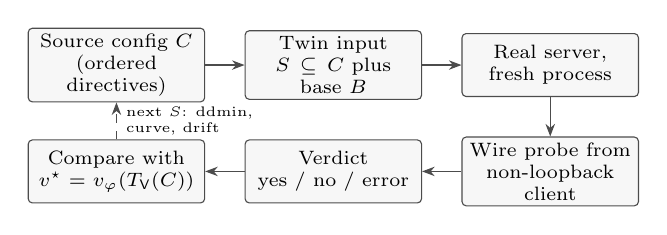
\begin{tikzpicture}[font=\scriptsize, node distance=2.5mm and 5mm,
  box/.style={draw=black!70, rounded corners=1.5pt, align=center, text width=21mm, minimum height=8mm, inner sep=2pt, fill=black!3},
  arr/.style={-{Stealth[length=1.6mm]}, draw=black!70}]
\node[box] (src) {Source config $C$\\(ordered directives)};
\node[box, right=of src] (sub) {Twin input\\$S\subseteq C$ plus base $B$};
\node[box, right=of sub] (srv) {Real server,\\fresh process};
\node[box, below=5mm of srv] (probe) {Wire probe from\\non-loopback client};
\node[box, left=of probe] (ver) {Verdict\\yes / no / error};
\node[box, left=of ver] (cmp) {Compare with\\$v^\star=v_\varphi(T_\Vb(C))$};
\draw[arr] (src) -- (sub);
\draw[arr] (sub) -- (srv);
\draw[arr] (srv) -- (probe);
\draw[arr] (probe) -- (ver);
\draw[arr] (ver) -- (cmp);
\draw[arr, dashed] (cmp) -- node[right, align=left, font=\tiny]{next $S$: ddmin,\\curve, drift} (src);
\end{tikzpicture}
\end{document}
